% !TEX root = ../geogebra-practices.tex
% Author: Alfredo Sánchez Alberca (asalber@ceu.es)
\chapter{Introduction to Geogebra}

\section{Introduction}
In the last decades, the computational power of computers have converted them in powerful tools for disciplines that, as Mathematics, require a large amount of complex computations.

Geogebra\footnote{These practices are based on version 6.0 of Classic Geogebra} is one of the most used programs for doing numerical and symbolic computations.
Beyond their capabilities for the numerical, vectorial and matrix calculus, it also makes graphical representations.
This allows to solve a lot of problems of Algebra, Analysis, Calculus, Geometry and even Statistics.
The advantage of Geogebra versus other software as Mathematica, Mapple or MATLAB, is its simplicity, what makes it suitable for teaching Maths, and that is open source software, so that it can be modified and installed for free.

\begin{center}
\includegraphics[scale=0.8]{img/introduction/geogebra-logo}
\end{center}

This software can be downloaded from the web \url{https://www.geogebra.org}.
There is also in this web an on-line version of the program that can be used as a web application without installing it in the computer.
This web also contains a lot of tutorials an educational resources available to the users.
In fact, any user can register an upload to this site activities developed with Geogebra.

The goal of this practice is to introduce to the student the basic usage of this program for Calculus.


\section{Starting the program}
As any other Windows applications, to start the program you have to click the \menu{Windows start} button and then select \menu{All the programs > Geogera} or simply double click the desktop shortcut icon \includegraphics[scale=0.04]{img/introduction/geogebra-icon} if there is one.

When the program starts, the initial windows is shown (figure \ref{g:start-window}), allowing the user to choose among different working environments or \emph{Perspectives}.

\begin{figure}[h!]
\begin{center}
\includegraphics[width=\textwidth]{img/introduction/start-window}
\caption{Starting perspective of Geogegra.} \label{g:start-window}
\end{center}
\end{figure}

\section{Views}
Geogebra provides several windows that are called \emph{Views} and different working environments called \emph{Perspectives} that combine some views.
Both views and perspectives can be activated in the main menu of Geogebra that appears in the top right corner.
The most important views that we are going to use during these practices are:
\begin{description}
\item[Algebraic View] \includegraphics[scale=0.03]{img/introduction/algebraic-view-icon} This view allows to make algebraic and geometric constructions.
      It provides an \field{Input Bar} where the user can enter command and algebraic expressions.
      This is view is active by default when the program starts.
\item[Graphic View] \includegraphics[scale=0.03]{img/introduction/graphics-view-icon}
      This view allows to represent graphically geometric objects in the real plane.
      Beside the algebraic view, this view is also active by default when the program starts.
\item[3D Graphics View] \includegraphics[scale=0.3]{img/introduction/3d-graphics-view-icon} This view allows to represent graphically geometric objects in the real space.
      This view is not activated by default when the program starts, so that it must be activated by the user when it is required.
\item[CAS View] \includegraphics[scale=0.03]{img/introduction/cas-view-icon} (Computer Algebra System) This view allows to do symbolic calculations.
      It provides an \field{Input Bar} similar to the one of the algebraic view where you can enter commands and mathematical expressions, and evaluate them.
      This view is not activated by default when the program starts, but \emph{it will be the most used view during these practices}.
\end{description}


\section{Expression edition in the \field{CAS View}}
Before doing any computation with a mathematica expression, you need to know how to enter that expression and learn to manage it.


\subsection*{Entering expressions}
Any mathematical expression must be entered in the \field{Input Bar} of the \field{CAS View} (figure~\ref{g:input-bar}).

\begin{figure}[h!]
\begin{center}
\includegraphics[scale=0.6]{img/introduction/input-bar}
\caption{Input Bar.} \label{g:input-bar}
\end{center}
\end{figure}

The \field{Input Bar} allows to enter mathematical expressions, commands and text annotations.
In the mathematical expressions we can enter numbers, roman letters, greek letters, mathematical operators and any symbols that appears in the virtual keyboard.
It also allows to enter \LaTeX\footnote{\url{https://www.latex-project.org/}} code to format expressions.
For instance, it is possible to write superscripts with the command \command{\^{}} and subscripts with the command \command{\_}.

When the key \command{Enter} is pressed after entering a mathematical expression, Geogebra tries to evaluate it and it shows the result of the evaluation just below the expression, or a warning when there is some mistake in the expression.

Them most common operators for the construction of mathematical expressions are shown in the table below.

\begin{center}
\begin{tabular}{cc}
\tcrule
\textbf{Symbol} & \textbf{Operator} \\
\command{+}     & Addition          \\
\command{-}     & Subtraction       \\
\command{*}     & Product           \\
\command{/}     & Division          \\
\command{\^{}}  & Power             \\
\bcrule
\end{tabular}
\end{center}

At the time of writing a mathematical expression, you must take into account that Geogebra has an order of priority to evaluate the operators.
First it evaluates predefined functions and constants, after powers, after products and quotients (both with the same priority and from left to right), and finally additions and subtractions (both with the same priority and from left to right).
To force the evaluation of a subexpression, skipping the order of priority, you must use parenthesis.
Thus, as it can be appreciated in the table below, depending on how a expression is entered, you can get different results.

\begin{center}\renewcommand{\arraystretch}{2}
\begin{tabular}{cc}
\tcrule
\textbf{Entered expression} & \textbf{Evaluated expression} \\
\texttt{4x-1/x-5}           & $4x-\dfrac{1}{x}-5$           \\
\texttt{(4x-1)/x-5}         & $\dfrac{4x-1}{x}-5$           \\
\texttt{4x-1/(x-5)}         & $4x-\dfrac{1}{x-5}$           \\
\texttt{(4x-1)/(x-5)}       & $\dfrac{4x-1}{x-5}$           \\
\bcrule
\end{tabular}
\end{center}

Every expression that is entered in the \field{CAS View} is labelled with a number that allows to identify it.
Later, every time that we want to reference that expression we can use that identifier instead of writing again the whole expression.

There are two ways of referring to an expression, that are the static and the dynamic references.
To do a static reference we must write the symbol \# followed by the identifier number of the expression.
On the other hand, to do a dynamic reference we must write the symbol \$ followed by the identifier number of the expression.
A static reference will not change the expression where the reference is done even when the original expression changes, while for a dynamic reference, when the original expression changes, that change will be reflected in the expression where the reference is done.

It is possible to select any expression or subexpression of the \field{CAS View} and then copy and paste it in the \field{Input Bar}.


\subsection*{Entering text notes}
Geogebra also allows to enter text notes or comments int he \field{Input Bar}.
For that you have to right-click the \field{Input Bar} and select the option \option{Text} in the contextual menu that appears.
Text annotations are very helpful to explain the steps in a mathematical construction or to interpret the results.


\subsection*{Removing expressions}
Of course, it is possible to remove a expression from the \field{CAS View}.
For that you have to go to the line with the expression to remove and click the button \includegraphics[scale=0.035]{img/introduction/bin-button.png} or right-click that line and select the option \option{Delete row} in the contextual menu that appears.

If sometime we commit a mistake entering or deleting a wrong expression, it is possible to undo the last operations or redo them clicking the buttons \includegraphics[scale=0.03]{img/introduction/undo-button.png} or \includegraphics[scale=0.03]{img/introduction/redo-button.png} respectively.


\subsection*{Defining variables}
To define a variable we can use roman letters or greek letters.
The name of a variable can have more than one letter and, in this case, it is also possible to use numbers but it must start always by a letter.
Thus, for Geogebra, the expression \command{xy}, is not interpreted as the product of the variables $x$ and $y$, but the variable $xy$.
In addition, it distinguishes between upper and lower case, so that $xy$ and $xY$ are different variables.


\subsection*{Defining constants and functions}
To define a constant or a function the definition operator \command{:=} must be used.
To define a constant you have to write the name of the constant followed by \command{:=} and the value of the constant.
For example, to define the gravity constant we have to write \command{g:=9.81}.

On the other hand, to define a function you have to write the name of the function, followed buy the list of variables separated by commas and between parenthesis, then \command{:=} and finally the expression that defines the function.
For example, to define the function that calculates the area of triangle with base $b$ and high $h$, we have to write \command{a(b,h):=(b*h)/2} (ver figure~\ref{g:expressions}).


\begin{figure}[h!]
\begin{center}
\includegraphics[scale=0.6]{img/introduction/math-expressions}
\caption{Entering mathematical expressions in the \field{Input Bar}.} \label{g:expressions}
\end{center}
\end{figure}


If we have defined a constant or function, and we change the definition after, the changes will be reflected in any other expression that contains the constant or function, except if the reference is static.

To remove a definition and free the name of the constant or function, for example \command{c}, we can use the command \command{Delete(c)} or the command \command{c:=}.


\subsection*{Predefined constants and functions}
Geogebra provides several predefined constants and functions that can be used in the mathematical expressions.
The sintax of some of these constants and functions is shown in the table~\ref{t:predefined-functions}, although, instead of using those commands, we can use the operators and constants of the virtual keyboard.

\begin{table}[h!]
\centering
\begin{tabular}{cl}
\tcrule
\textbf{Sintaxis}   & \textbf{Constante o función}                 \\
\command{pi}        & The number $\pi=3.14159\ldots$               \\
\command{Alt+e}     & Euler's constant $e=2.71828\ldots$           \\
\command{Alt+i}     & Imaginary number $i=\sqrt{-1}$               \\
\command{inf}       & Infinity $\infty$                            \\
\command{exp(x)}    & Exponential function $e^x$                   \\
\command{log(a,x)}  & Logarithmic function of base $a$, $\log_a x$ \\
\command{ln(x)}     & Neperian logarithmic function $\ln x$        \\
\command{sqrt(x)}   & Square root function $\sqrt{x}$              \\
\command{sin(x)}    & Sine function $\sin x$                       \\
\command{cos(x)}    & Cosine function $\cos x$                     \\
\command{tan(x)}    & Tangent function $\tan x$                    \\
\command{arcsin(x)} & Arcsine function $\arcsin x$                 \\
\command{arccos(x)} & Arccosine function $\arccos x$               \\
\command{arctan(x)} & Arctangent function $\arctan x$              \\
\bcrule
\end{tabular}
\caption{Sintax of some predefined constants and functions in Geogebra.} \label{t:predefined-functions}
\end{table}


\subsection*{Entering vectors and matrices}
Geogebra allows also to handle vectors and matrices.
To define a vector you must write its coordinates separated by commas between parenthesis.
For example, to enter the vector $(x,y,z)$ we have to write \command{(x,y,z)} (see figure~\ref{g:expressions}).

To define a matrix you must enter its elements by rows, separated by commas and between curly brackets.
For example, to enter the matrix
\[
\left(
\begin{array}{ccc}
1 & 2 & 3 \\
a & b & c \\
\end{array}
\right)
\]
we have to write \command{\{\{1,2,3\},\{a,b,c\}\}} (see figure~\ref{g:expressions}).


\subsection*{Simplifying expressions}
By default Geogebra always tries to simplify the mathematical expressions when it evaluates them.
For example, if you enter $x+x$ the result will be $2x$.
To avoid simplification you can change to the \button{Keep Input} mode clicking the button \includegraphics[scale=0.03]{img/introduction/keep-input-button}.

However, when Geogebra evaluates a mathematical expression it does not perform more complex simplifications, like, for instance, the simplification $\sin(x)^2+\cos(x)^2=1$.
To do this there are three commands:
\begin{description}
\item[Simplify] This is the most simple and tries to simplify a mathematical expression the most.
      For example, the command \command{Simplify(sin(x)\^{}2+cos(x)\^{}2)} returns \result{1}.
\item[Expand] This command tries to expand a mathematical expression computing all the possible powers, products, quotients, additions and subtractions.
      For example, the command \command{Expand((x+1)\^{}2)} returns \result{x\^{}2+2x+1}.
\item[Factor] This command tries to factorize a mathematical expression.
      For example, the command \command{Factoriza(x\^{}2+2x+1)} returns \result{(x+1)\^{}2}.
\end{description}

In any of these simplifications Geogebra uses by default the exact mode and returns fractional expressions.
To get the approximate value of a mathematical expression, with decimals, we must change to the \button{Numeric Evaluation} mode clicking the button \includegraphics[scale=0.03]{img/introduction/approximate-button}.
The number of decimal places showed can be set in the settings menu of Geogebra.

Lastly, it is possible to replace any variable by a value with the command \command{Substitute(<Expression>, <Substitution list>)}.
For example, the command \command{Substitute(2x+y, x=2, y=1)} returns \result{5}.


\subsection*{Entering equations and inequations}
To define equations in Geogebra the equality symbol \command{=} must be used.
Por example, the command \command{2x-y=1} defines the equation of a line.

And to define inequations we can use the symbols less than \command{<}, greater than \command{>}, less than or equal to \command{<=} or greater than or equal to \command{>=}.
For example, the command \command{x\^{}2+y\^{}2<=1} defines the circle with radius 1 centered at the origin.

To solve equations and inequation you can use the command \command{Solve(<equations>)}.
For example, the command \command{Solve(x\^{}2-5x+4=0)} returns \result{\{x=1, x=4\}}.
It is also possible to impose restrictions for the variables.
For example, the command \command{Solve(x\^{}2-5x+4=0, x>3)} returns only the solution \result{\{x=4\}}.

To solve systems of equations you must enter the list of equations separated by commans and between curly brackets.
For example, the command \command{Solve({2x+3=7, x-y=-1})} returns \result{\{x=3, y=2\}}.

This command also solves inequations.
For example, the command \command{Solve(3x-2<1)} returns \result{\{x<1\}}.


\section{Graphical representations}
One of the strengths of Geogebra is its graphics capabilities, sice it allows to represent graphically a lot of geometric objects both in the plane and in the real space.


\subsection*{Graphical representations in the real plane}
To represent geometric objects in the real plane $\mathbb{R}^2$, Geogebra uses the \field{Graphics View}.
By default any function defined in the \field{CAS View} will be plotted in this view.
To graphically represent other objects like constants, equations or inequations, it is required to click on the circle that appears to the left of the expression (see figure~\ref{g:graphics-view}).
To hide back the object in the \field{Graphics View} you have to click again on this circle.

\begin{figure}[h!]
\begin{center}
\includegraphics[width=\textwidth]{img/introduction/graphic-view}
\caption{Graphical representations in the \field{Graphics View}.} \label{g:graphics-view}
\end{center}
\end{figure}

Geogebra allows also the graphical representation of parametric functions defining the vector with the coordinate functions depending on one parameter.
For example, the command \command{g(t):=(cos(t), 2sin(t)cos(t))} plots the curve of the figure~\ref{g:parametric-curve}.

\begin{figure}[h!]
\begin{center}
\includegraphics[width=\textwidth]{img/introduction/parametric-curve}
\caption{Graphical representation of a parametric curve in the real plane.} \label{g:parametric-curve}
\end{center}
\end{figure}

It is possible to change the aspect of any geometric object right-clicking on it and selecting the option \option{Settings} in the contextual menu that appears.
This opens a panel that allows to change the name of the object, the colour, the thickness or the opacity of the line, or even to enter a label that will appear next to the object in the \field{Graphics View}.

The \field{Graphics View} is centered at the origin of coordinates by default, but it is possible to make a zoom in or out clicking on the buttons \includegraphics[scale=0.03]{img/introduction/zoom-in-button} and \includegraphics[scale=0.03]{img/introduction/zoom-out-button} respectively.
It is also possible to move the view clicking at any position in the view and dragging the mouse.
To come back to the original view you can click on the button \includegraphics[scale=0.03]{img/introduction/home-button}.


\subsection*{Graphical representations in the real space}
To represent geometric objects in the real space $\mathbb{R}^3$, Geogebra uses the \field{3D Graphics View}.

By default, any function of two variables defined in the \field{CAS View} will be plotted in this view.
To graphically represent other objects like equations it is required to click on the circle that appears to the left of the expression (see figure~\ref{g:3D-graphics-view}).
Para ocultar de nuevo el objeto en la \field{Graphics View} basta con volver a hacer clic sobre ese círculo.

\begin{figure}[h!]
\begin{center}
\includegraphics[width=\textwidth]{img/introduction/3D-graphic-view}
\caption{Grahpical representations in the \field{3D Graphics View}.} \label{g:3D-graphics-view}
\end{center}
\end{figure}

The same than in the \field{Graphics View} it is also possible to represent parametric functions defining the vector with the coordinate functions depending on one parameter.
For example, the command \command{h(t):=(cos(t), sin(t), t/2)} plots the curve of figure~\ref{g:3D-parametric-curve}.

\begin{figure}[h!]
\begin{center}
\includegraphics[width=\textwidth]{img/introduction/3D-parametric-curve}
\caption{Graphical representation of a parametric curve in the real space.} \label{g:3D-parametric-curve}
\end{center}
\end{figure}

The same than in the \field{Graphics View}, it is possible to change the aspect of any geometric object right-clicking on it and selecting the option \option{Settings} in the contextual menu that appears.
This opens a panel that allows to change the name of the object, the colour, the thickness or the opacity of the line, or even to enter a label that will appear next to the object in the \field{3D Graphics View}.

In the same way, it is possible to make a zoom in or out clicking on the buttons \includegraphics[scale=0.03]{img/introduction/zoom-in-button} and \includegraphics[scale=0.03]{img/introduction/zoom-out-button} respectively.
It is also possible to move the view with the button \includegraphics[scale=0.03]{img/introduction/move-button} or to rotate it with the button \includegraphics[scale=0.03]{img/introduction/rotate-button}.


\section{File management}
The mathematical expressions and calculus of the \field{CAS View} and the graphics of the \field{Graphics View} and \field{3D Graphics View} can be saved into a file.

\subsection*{Saving a file}
To save the mathematical expressions, calculus and graphics of a working session you must select the menu \menu{File>Save}.
If you have not logged in to the Geogebra web site a dialog appears asking for the user name an password to log in (see figure~\ref{g:login}).
If the you has no account in this site now is possible to register, but if you do not want to log in just click the link \button{Continue without signing in now}.

\begin{figure}[h!]
\begin{center}
\includegraphics[scale=0.6]{img/introduction/login}
\caption{Login dialog of Geogebra web site.} \label{g:login}
\end{center}
\end{figure}

If you have logged in to the Geogebra web site, it will ask for the file name and the file will be uploaded to the Geogebra web site.
This way the file will be available whenever we are connected to this site with our user account.

If you have not logged in to the Geogebra web site, then a dialog is shown where you can enter the file name and select the local folder where to save the file in your computer.
Geogebras' files have extension \texttt{*.ggb}.

Once the file is saved, its name will appear in the title bar of the Geogebra window.


\subsubsection*{Opening a file}
To open a file in Geogebra you can use the menu \menu{File>Open}.
In the dialog shown you can choose to open a file from the Geogebra web site or to open a local file.

If you has logged in to the Geogebra web site, the files saved in our user account will appear automatically.
Eve if you are not logged in, you can open any public file in the Geogebra cloud.
For that we can search for a file entering a keyword in the search bar and Geogebra will show a list with all the files that contains that word.
Selecting any of them will download the file and open it.

If you want to open a local file you have to click on the folder icon.
This will open a dialog where you can select the file to open.


% \section{Printing}
% Geogebra permite imprimir las vistas gráficas seleccionando el menú \menu{Previsualización}.
% Tras esto aparece un cuadro de diálogo donde se puede seleccionar la ventana gráfica que se desea imprimir and las unidades de los ejes.
% Finalmente aparece el cuadro de diálogo de las impresoras donde hay que seleccionar la impresora con la que se quiere imprimir.

% También es posible exportar las vistas gráficas a diferentes formatos con el menú \menu{Descargar como}.
% Si se desea imprimir además de las gráficos las expresiones de la \field{CAS View} hay que seleccionar la opción \option{Construcción dinámica con página web (html)}.
% Esto genera una página web que puede abrirse con cualquier navegador and después imprimirse de la forma habitual.


\section{Solved exercises}
\begin{enumerate}
\item Enter and evaluate the following expressions.
      \begin{enumerate}
      \item $4x-\dfrac{1}{x}-5$.
            \begin{indication}
            Enter the expression \command{4x-1/x-5} in the \field{Input Bar} of the \field{CAS View}.
            \end{indication}
      \item $\dfrac{4x-1}{x}-5$.
            \begin{indication}
            Enter the expression \command{(4x-1)/x-5} in the \field{Input Bar} of the \field{CAS View}.
            \end{indication}
      \item $4x-\dfrac{1}{x-5}$.
            \begin{indication}
            Enter the expression \command{4x-1/(x-5)} in the \field{Input Bar} of the \field{CAS View}.
            \end{indication}
      \item $\dfrac{4x-1}{x-5}$.
            \begin{indication}
            Enter the expression \command{(4x-1)/(x-5)} in the \field{Input Bar} of the \field{CAS View}.
            \end{indication}
      \end{enumerate}

\item Define the following mathematical objects and plot them.
      \begin{enumerate}
      \item The constants $a=2$ and $b=3$.
            \begin{indication}
            \begin{enumerate}
            \item Enter the command \command{a:=2} in the \field{Input Bar} of the \field{CAS View} and activate the \field{Graphics View}.
            \item To plot the slider of the constant click the circle that appears to the left of the previous expression.
            \item Enter the command \command{b:=3} in the \field{Input Bar}.
            \item To plot the slider of the constant click the circle that appears to the left of the previous expression.
            \end{enumerate}
            \end{indication}
      \item The line $f(x)=a+bx$.
            Use the sliders of the constants to see how the line changes.
            \begin{indication}
            Enter the command \command{f(x):=a+b*x} in the \field{Input Bar}.
            \end{indication}
      \item The equation $ax^2+by^2=8$.
            Use the sliders of the constants to see how the conic changes.
            \begin{indication}
            Enter the command \command{a*x\^{}2+b*y\^{}2=8} in the \field{Input Bar}.
            \end{indication}
      \end{enumerate}

\item Define the following functions and plot them.
      \begin{enumerate}
      \item $f(x):=x^2$.
            \begin{indication}
            Enter the command \command{f(x):=x\^{}2} in the \field{Input Bar} of the \field{CAS View} and activate the \field{Graphics View}.
            \end{indication}
      \item $g(x):=\log(x)$.
            \begin{indication}
            Enter the command \command{g(x):=log(x)} in the \field{Input Bar}.
            \end{indication}
      \item $h(x):=\sin(x)$.
            \begin{indication}
            Enter the command \command{g(x):=sin(x)} in the \field{Input Bar}.
            \end{indication}
      \item $g\circ f(x)$.
            \begin{indication}
            Enter the command \command{g(f(x))} in the \field{Input Bar} and click the circle that appears to the left of the expression.
            \end{indication}
      \item $h\circ g \circ f(x)$.
            \begin{indication}
            Enter the command \command{h(g(f(x)))} in the \field{Input Bar} and click the circle that appears to the left of the expression.
            \end{indication}
      \item $f\circ g \circ h(x)$.
            \begin{indication}
            Enter the command \command{f(g(h(x)))} in the \field{Input Bar} and click the circle that appears to the left of the expression.
            \end{indication}
      \end{enumerate}

\item Given the matrices
      \[
      A=\left(
      \begin{array}{cc}
      a_{11} & a_{12} \\
      a_{21} & a_{22} \\
      a_{31} & a_{32}
      \end{array}
      \right)
      \qquad
      B=\left(
      \begin{array}{ccc}
      1 & 2 & 3 \\
      4 & 5 & 6
      \end{array}
      \right)
      \]
      and the vector $\mathbf{v}=(x, y, z)$, se pide:

      \begin{enumerate}
      \item Define the matrices $A$ and $B$, and the vector $v$.
            \begin{indication}
            \begin{enumerate}
            \item Enter the command \command{A:=\{\{a\_{11},a\_{12}\},\{a\_{21},a\_{22}\},\{a\_{31},a\_{32}\}\}} in the \field{Input Bar} of the \field{CAS View}.
            \item Enter the command \command{B:=\{\{1,2,3\},\{4,5,6\}\}} in the \field{Input Bar}.
            \item Enter the command \command{v:=(x,y,z)} in the \field{Input Bar}.
            \end{enumerate}
            \end{indication}
      \item Compute $A\cdot B$.
            \begin{indication}
            Enter the command \command{A*B} in the \field{Input Bar}.
            \end{indication}
      \item Compute $B\cdot A$.
            \begin{indication}
            Enter the command \command{B*A} in the \field{Input Bar}.
            \end{indication}
      \item Compute $\mathbf{v}\cdot A$.
            \begin{indication}
            Enter the command \command{v*A} in the \field{Input Bar}.
            \end{indication}
      \item Compute $B\cdot \mathbf{v}$.
            \begin{indication}
            Enter the command \command{B*v} in the \field{Input Bar}.
            \end{indication}
      \item Substitute $x=1$, $y=1$ and $z=0$ in the previous vector and plot it.
            \begin{indication}
            Enter the command \command{Substitute(\$,\{x=1,y=1,z=0\})} in the \field{Input Bar} and click the circle that appears to the left of the expression.
            \end{indication}
      \item Compute the modulus of the previous vector.
            \begin{indication}
            Enter the command \command{|\$|} in the \field{Input Bar} and click the circle that appears to the left of the expression.
            \end{indication}
      \item Change the previous substitution for $x=0$, $y=0$ and $z=1$ and observe how changes the modulus of the previous vector.
            \begin{indication}
            Edit the line with the substitution and change it for \command{Substitute(\$,\{x=0,y=0,z=1\})} in the \field{Input Bar}.
            \end{indication}
      \end{enumerate}

\item Find out the points where the graphs of the functions $f(x)=x^2$ and $g(x)=\dfrac{x+1}{2}$ intersect and plot them.
      \begin{enumerate}
      \item Enter the command \command{f(x):=x\^{}2} in the \field{Input Bar} of the \field{CAS View} and activate the \field{Graphics View}.
      \item Enter the command \command{g(x):=(x+1)/2} in the \field{Input Bar}.
      \item To solve the equation, enter the command \command{Solve(f=g)} in the \field{Input Bar}.
      \item To plot the intersection points, enter the command \command{Intersect(f,g)} in the \field{Input Bar} and click on the circle that appears to the left of the expression.
      \end{enumerate}

\item Plot the parametric function
      \[
      g(t)=
      \begin{cases}
      \cos(t) \\
      2\sin(t)\cos(t)
      \end{cases}
      t\in \mathbb{R}
      \]

      \begin{indication}
      Enter the command \command{g(t):=(cos(t), 2sin(t)cos(t))} in the \field{Input Bar} of the \field{CAS View} and activate the \field{Graphics View}.
      \end{indication}

\item Plot the following surfaces
      \[
      f(x,y)=\dfrac{2\sin(x^2+y^2)}{\sqrt{x^2+y^2}}, \qquad x^2+y 2+(z-2)^2=1
      \]
      and and the parametric curve
      \[
      h(t)=
      \begin{cases}
      \sin(t) \\
      \cos(t) \\
      t/2
      \end{cases}
      t\in \mathbb{R}
      \]
      \begin{indication}
      \begin{enumerate}
      \item Enter the command \command{f(x,y):=2sin(x\^{}2+y\^{}2)/sqrt(x\^{}2+y\^{}2)} in the \field{Input Bar} of the \field{CAS View} and activate the \field{3D Graphics View}.
      \item Enter the command \command{x\^{}2+y\^{}2+(z-2)\^{}2=1}  in the \field{Input Bar}.
      \item Enter the command \command{h(t):=(sin(t),cos(t),t/2)}  in the \field{Input Bar}.
      \end{enumerate}
      \end{indication}
\end{enumerate}